% Graphic for TeX using PGF
% Title: S:\Senior Project\seniorProject2-2020-21-Docs\figs\dia\systemOperationFlowchart.dia
% Creator: Dia v0.97.2
% CreationDate: Wed Nov 25 16:20:30 2020
% For: Jason Braker
% \usepackage{tikz}
% The following commands are not supported in PSTricks at present
% We define them conditionally, so when they are implemented,
% this pgf file will use them.
\ifx\du\undefined
  \newlength{\du}
\fi
\setlength{\du}{15\unitlength}
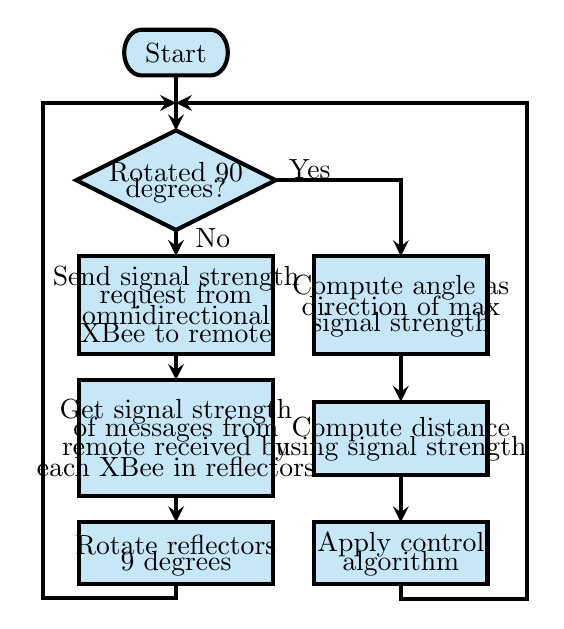
\begin{tikzpicture}[scale=0.55]
\pgftransformxscale{1.000000}
\pgftransformyscale{-1.000000}
\definecolor{dialinecolor}{rgb}{0.000000, 0.000000, 0.000000}
\pgfsetstrokecolor{dialinecolor}
\definecolor{dialinecolor}{rgb}{1.000000, 1.000000, 1.000000}
\pgfsetfillcolor{dialinecolor}
\pgfsetlinewidth{0.100000\du}
\pgfsetdash{}{0pt}
\pgfsetdash{}{0pt}
\pgfsetbuttcap
\pgfsetmiterjoin
\pgfsetlinewidth{0.100000\du}
\pgfsetbuttcap
\pgfsetmiterjoin
\pgfsetdash{}{0pt}
\definecolor{dialinecolor}{rgb}{0.780392, 0.905882, 0.968627}
\pgfsetfillcolor{dialinecolor}
\pgfpathmoveto{\pgfpoint{22.956946\du}{4.485162\du}}
\pgfpathlineto{\pgfpoint{25.983196\du}{4.485162\du}}
\pgfpathcurveto{\pgfpoint{26.401035\du}{4.485162\du}}{\pgfpoint{26.739759\du}{4.932877\du}}{\pgfpoint{26.739759\du}{5.485162\du}}
\pgfpathcurveto{\pgfpoint{26.739759\du}{6.037447\du}}{\pgfpoint{26.401035\du}{6.485162\du}}{\pgfpoint{25.983196\du}{6.485162\du}}
\pgfpathlineto{\pgfpoint{22.956946\du}{6.485162\du}}
\pgfpathcurveto{\pgfpoint{22.539108\du}{6.485162\du}}{\pgfpoint{22.200384\du}{6.037447\du}}{\pgfpoint{22.200384\du}{5.485162\du}}
\pgfpathcurveto{\pgfpoint{22.200384\du}{4.932877\du}}{\pgfpoint{22.539108\du}{4.485162\du}}{\pgfpoint{22.956946\du}{4.485162\du}}
\pgfusepath{fill}
\definecolor{dialinecolor}{rgb}{0.000000, 0.000000, 0.000000}
\pgfsetstrokecolor{dialinecolor}
\pgfpathmoveto{\pgfpoint{22.956946\du}{4.485162\du}}
\pgfpathlineto{\pgfpoint{25.983196\du}{4.485162\du}}
\pgfpathcurveto{\pgfpoint{26.401035\du}{4.485162\du}}{\pgfpoint{26.739759\du}{4.932877\du}}{\pgfpoint{26.739759\du}{5.485162\du}}
\pgfpathcurveto{\pgfpoint{26.739759\du}{6.037447\du}}{\pgfpoint{26.401035\du}{6.485162\du}}{\pgfpoint{25.983196\du}{6.485162\du}}
\pgfpathlineto{\pgfpoint{22.956946\du}{6.485162\du}}
\pgfpathcurveto{\pgfpoint{22.539108\du}{6.485162\du}}{\pgfpoint{22.200384\du}{6.037447\du}}{\pgfpoint{22.200384\du}{5.485162\du}}
\pgfpathcurveto{\pgfpoint{22.200384\du}{4.932877\du}}{\pgfpoint{22.539108\du}{4.485162\du}}{\pgfpoint{22.956946\du}{4.485162\du}}
\pgfusepath{stroke}
% setfont left to latex
\definecolor{dialinecolor}{rgb}{0.000000, 0.000000, 0.000000}
\pgfsetstrokecolor{dialinecolor}
\node at (24.470071\du,5.525162\du){Start};
\pgfsetlinewidth{0.100000\du}
\pgfsetdash{}{0pt}
\pgfsetdash{}{0pt}
\pgfsetbuttcap
{
\definecolor{dialinecolor}{rgb}{0.000000, 0.000000, 0.000000}
\pgfsetfillcolor{dialinecolor}
% was here!!!
\pgfsetarrowsend{stealth}
\definecolor{dialinecolor}{rgb}{0.000000, 0.000000, 0.000000}
\pgfsetstrokecolor{dialinecolor}
\draw (24.470071\du,13.253697\du)--(24.470071\du,14.388015\du);
}
\pgfsetlinewidth{0.100000\du}
\pgfsetdash{}{0pt}
\pgfsetdash{}{0pt}
\pgfsetbuttcap
{
\definecolor{dialinecolor}{rgb}{0.000000, 0.000000, 0.000000}
\pgfsetfillcolor{dialinecolor}
% was here!!!
\pgfsetarrowsend{stealth}
\definecolor{dialinecolor}{rgb}{0.000000, 0.000000, 0.000000}
\pgfsetstrokecolor{dialinecolor}
\draw (24.470071\du,6.485162\du)--(24.470071\du,8.891787\du);
}
\pgfsetlinewidth{0.100000\du}
\pgfsetdash{}{0pt}
\pgfsetdash{}{0pt}
\pgfsetmiterjoin
\pgfsetbuttcap
{
\definecolor{dialinecolor}{rgb}{0.000000, 0.000000, 0.000000}
\pgfsetfillcolor{dialinecolor}
% was here!!!
\pgfsetarrowsend{stealth}
{\pgfsetcornersarced{\pgfpoint{0.000000\du}{0.000000\du}}\definecolor{dialinecolor}{rgb}{0.000000, 0.000000, 0.000000}
\pgfsetstrokecolor{dialinecolor}
\draw (24.470071\du,28.756650\du)--(24.470071\du,29.380791\du)--(18.662017\du,29.380791\du)--(18.662017\du,7.688475\du)--(24.470071\du,7.688475\du);
}}
\pgfsetlinewidth{0.100000\du}
\pgfsetdash{}{0pt}
\pgfsetdash{}{0pt}
\pgfsetmiterjoin
\pgfsetbuttcap
{
\definecolor{dialinecolor}{rgb}{0.000000, 0.000000, 0.000000}
\pgfsetfillcolor{dialinecolor}
% was here!!!
\pgfsetarrowsend{stealth}
{\pgfsetcornersarced{\pgfpoint{0.000000\du}{0.000000\du}}\definecolor{dialinecolor}{rgb}{0.000000, 0.000000, 0.000000}
\pgfsetstrokecolor{dialinecolor}
\draw (28.831982\du,11.072742\du)--(28.831982\du,11.079441\du)--(34.317833\du,11.079441\du)--(34.317833\du,14.401811\du);
}}
% setfont left to latex
\definecolor{dialinecolor}{rgb}{0.000000, 0.000000, 0.000000}
\pgfsetstrokecolor{dialinecolor}
\node[anchor=west] at (28.920363\du,10.565993\du){Yes};
% setfont left to latex
\definecolor{dialinecolor}{rgb}{0.000000, 0.000000, 0.000000}
\pgfsetstrokecolor{dialinecolor}
\node[anchor=west] at (24.833774\du,13.604637\du){No};
\definecolor{dialinecolor}{rgb}{0.780392, 0.905882, 0.968627}
\pgfsetfillcolor{dialinecolor}
\fill (20.230538\du,19.822333\du)--(20.230538\du,24.922333\du)--(28.709605\du,24.922333\du)--(28.709605\du,19.822333\du)--cycle;
\pgfsetlinewidth{0.100000\du}
\pgfsetdash{}{0pt}
\pgfsetdash{}{0pt}
\pgfsetmiterjoin
\definecolor{dialinecolor}{rgb}{0.000000, 0.000000, 0.000000}
\pgfsetstrokecolor{dialinecolor}
\draw (20.230538\du,19.822333\du)--(20.230538\du,24.922333\du)--(28.709605\du,24.922333\du)--(28.709605\du,19.822333\du)--cycle;
% setfont left to latex
\definecolor{dialinecolor}{rgb}{0.000000, 0.000000, 0.000000}
\pgfsetstrokecolor{dialinecolor}
\node at (24.470071\du,21.212333\du){Get signal strength};
% setfont left to latex
\definecolor{dialinecolor}{rgb}{0.000000, 0.000000, 0.000000}
\pgfsetstrokecolor{dialinecolor}
\node at (24.470071\du,22.012333\du){of messages from};
% setfont left to latex
\definecolor{dialinecolor}{rgb}{0.000000, 0.000000, 0.000000}
\pgfsetstrokecolor{dialinecolor}
\node at (24.470071\du,22.812333\du){remote received by};
% setfont left to latex
\definecolor{dialinecolor}{rgb}{0.000000, 0.000000, 0.000000}
\pgfsetstrokecolor{dialinecolor}
\node at (24.470071\du,23.612333\du){each XBee in reflectors};
\definecolor{dialinecolor}{rgb}{0.780392, 0.905882, 0.968627}
\pgfsetfillcolor{dialinecolor}
\fill (24.470071\du,8.891787\du)--(28.831982\du,11.072742\du)--(24.470071\du,13.253697\du)--(20.108161\du,11.072742\du)--cycle;
\pgfsetlinewidth{0.100000\du}
\pgfsetdash{}{0pt}
\pgfsetdash{}{0pt}
\pgfsetmiterjoin
\definecolor{dialinecolor}{rgb}{0.000000, 0.000000, 0.000000}
\pgfsetstrokecolor{dialinecolor}
\draw (24.470071\du,8.891787\du)--(28.831982\du,11.072742\du)--(24.470071\du,13.253697\du)--(20.108161\du,11.072742\du)--cycle;
% setfont left to latex
\definecolor{dialinecolor}{rgb}{0.000000, 0.000000, 0.000000}
\pgfsetstrokecolor{dialinecolor}
\node at (24.470071\du,10.712742\du){Rotated 90};
% setfont left to latex
\definecolor{dialinecolor}{rgb}{0.000000, 0.000000, 0.000000}
\pgfsetstrokecolor{dialinecolor}
\node at (24.470071\du,11.512742\du){degrees?};
\definecolor{dialinecolor}{rgb}{0.780392, 0.905882, 0.968627}
\pgfsetfillcolor{dialinecolor}
\fill (30.525333\du,14.401811\du)--(30.525333\du,18.701811\du)--(38.110333\du,18.701811\du)--(38.110333\du,14.401811\du)--cycle;
\pgfsetlinewidth{0.100000\du}
\pgfsetdash{}{0pt}
\pgfsetdash{}{0pt}
\pgfsetmiterjoin
\definecolor{dialinecolor}{rgb}{0.000000, 0.000000, 0.000000}
\pgfsetstrokecolor{dialinecolor}
\draw (30.525333\du,14.401811\du)--(30.525333\du,18.701811\du)--(38.110333\du,18.701811\du)--(38.110333\du,14.401811\du)--cycle;
% setfont left to latex
\definecolor{dialinecolor}{rgb}{0.000000, 0.000000, 0.000000}
\pgfsetstrokecolor{dialinecolor}
\node at (34.317833\du,15.791811\du){Compute angle as};
% setfont left to latex
\definecolor{dialinecolor}{rgb}{0.000000, 0.000000, 0.000000}
\pgfsetstrokecolor{dialinecolor}
\node at (34.317833\du,16.591811\du){direction of max};
% setfont left to latex
\definecolor{dialinecolor}{rgb}{0.000000, 0.000000, 0.000000}
\pgfsetstrokecolor{dialinecolor}
\node at (34.317833\du,17.391811\du){signal strength};
\definecolor{dialinecolor}{rgb}{0.780392, 0.905882, 0.968627}
\pgfsetfillcolor{dialinecolor}
\fill (30.525333\du,20.777419\du)--(30.525333\du,23.968519\du)--(38.110333\du,23.968519\du)--(38.110333\du,20.777419\du)--cycle;
\pgfsetlinewidth{0.100000\du}
\pgfsetdash{}{0pt}
\pgfsetdash{}{0pt}
\pgfsetmiterjoin
\definecolor{dialinecolor}{rgb}{0.000000, 0.000000, 0.000000}
\pgfsetstrokecolor{dialinecolor}
\draw (30.525333\du,20.777419\du)--(30.525333\du,23.968519\du)--(38.110333\du,23.968519\du)--(38.110333\du,20.777419\du)--cycle;
% setfont left to latex
\definecolor{dialinecolor}{rgb}{0.000000, 0.000000, 0.000000}
\pgfsetstrokecolor{dialinecolor}
\node at (34.317833\du,22.012969\du){Compute distance};
% setfont left to latex
\definecolor{dialinecolor}{rgb}{0.000000, 0.000000, 0.000000}
\pgfsetstrokecolor{dialinecolor}
\node at (34.317833\du,22.812969\du){using signal strength};
\definecolor{dialinecolor}{rgb}{0.780392, 0.905882, 0.968627}
\pgfsetfillcolor{dialinecolor}
\fill (30.525333\du,26.058941\du)--(30.525333\du,28.758941\du)--(38.110333\du,28.758941\du)--(38.110333\du,26.058941\du)--cycle;
\pgfsetlinewidth{0.100000\du}
\pgfsetdash{}{0pt}
\pgfsetdash{}{0pt}
\pgfsetmiterjoin
\definecolor{dialinecolor}{rgb}{0.000000, 0.000000, 0.000000}
\pgfsetstrokecolor{dialinecolor}
\draw (30.525333\du,26.058941\du)--(30.525333\du,28.758941\du)--(38.110333\du,28.758941\du)--(38.110333\du,26.058941\du)--cycle;
% setfont left to latex
\definecolor{dialinecolor}{rgb}{0.000000, 0.000000, 0.000000}
\pgfsetstrokecolor{dialinecolor}
\node at (34.317833\du,27.048941\du){Apply control};
% setfont left to latex
\definecolor{dialinecolor}{rgb}{0.000000, 0.000000, 0.000000}
\pgfsetstrokecolor{dialinecolor}
\node at (34.317833\du,27.848941\du){algorithm};
\pgfsetlinewidth{0.100000\du}
\pgfsetdash{}{0pt}
\pgfsetdash{}{0pt}
\pgfsetbuttcap
{
\definecolor{dialinecolor}{rgb}{0.000000, 0.000000, 0.000000}
\pgfsetfillcolor{dialinecolor}
% was here!!!
\pgfsetarrowsend{stealth}
\definecolor{dialinecolor}{rgb}{0.000000, 0.000000, 0.000000}
\pgfsetstrokecolor{dialinecolor}
\draw (24.470071\du,18.688015\du)--(24.470071\du,19.822333\du);
}
\pgfsetlinewidth{0.100000\du}
\pgfsetdash{}{0pt}
\pgfsetdash{}{0pt}
\pgfsetbuttcap
{
\definecolor{dialinecolor}{rgb}{0.000000, 0.000000, 0.000000}
\pgfsetfillcolor{dialinecolor}
% was here!!!
\pgfsetarrowsend{stealth}
\definecolor{dialinecolor}{rgb}{0.000000, 0.000000, 0.000000}
\pgfsetstrokecolor{dialinecolor}
\draw (24.470071\du,24.922333\du)--(24.470071\du,26.056650\du);
}
\pgfsetlinewidth{0.100000\du}
\pgfsetdash{}{0pt}
\pgfsetdash{}{0pt}
\pgfsetbuttcap
{
\definecolor{dialinecolor}{rgb}{0.000000, 0.000000, 0.000000}
\pgfsetfillcolor{dialinecolor}
% was here!!!
\pgfsetarrowsend{stealth}
\definecolor{dialinecolor}{rgb}{0.000000, 0.000000, 0.000000}
\pgfsetstrokecolor{dialinecolor}
\draw (34.317833\du,18.701811\du)--(34.317833\du,20.777419\du);
}
\pgfsetlinewidth{0.100000\du}
\pgfsetdash{}{0pt}
\pgfsetdash{}{0pt}
\pgfsetbuttcap
{
\definecolor{dialinecolor}{rgb}{0.000000, 0.000000, 0.000000}
\pgfsetfillcolor{dialinecolor}
% was here!!!
\pgfsetarrowsend{stealth}
\definecolor{dialinecolor}{rgb}{0.000000, 0.000000, 0.000000}
\pgfsetstrokecolor{dialinecolor}
\draw (34.317833\du,23.968519\du)--(34.317833\du,26.058941\du);
}
\pgfsetlinewidth{0.100000\du}
\pgfsetdash{}{0pt}
\pgfsetdash{}{0pt}
\pgfsetmiterjoin
\pgfsetbuttcap
{
\definecolor{dialinecolor}{rgb}{0.000000, 0.000000, 0.000000}
\pgfsetfillcolor{dialinecolor}
% was here!!!
\pgfsetarrowsend{stealth}
{\pgfsetcornersarced{\pgfpoint{0.000000\du}{0.000000\du}}\definecolor{dialinecolor}{rgb}{0.000000, 0.000000, 0.000000}
\pgfsetstrokecolor{dialinecolor}
\draw (34.317833\du,28.758941\du)--(34.317833\du,29.400791\du)--(39.852453\du,29.400791\du)--(39.852453\du,7.688475\du)--(24.470071\du,7.688475\du);
}}
\definecolor{dialinecolor}{rgb}{0.780392, 0.905882, 0.968627}
\pgfsetfillcolor{dialinecolor}
\fill (20.230538\du,14.388015\du)--(20.230538\du,18.688015\du)--(28.709605\du,18.688015\du)--(28.709605\du,14.388015\du)--cycle;
\pgfsetlinewidth{0.100000\du}
\pgfsetdash{}{0pt}
\pgfsetdash{}{0pt}
\pgfsetmiterjoin
\definecolor{dialinecolor}{rgb}{0.000000, 0.000000, 0.000000}
\pgfsetstrokecolor{dialinecolor}
\draw (20.230538\du,14.388015\du)--(20.230538\du,18.688015\du)--(28.709605\du,18.688015\du)--(28.709605\du,14.388015\du)--cycle;
% setfont left to latex
\definecolor{dialinecolor}{rgb}{0.000000, 0.000000, 0.000000}
\pgfsetstrokecolor{dialinecolor}
\node at (24.470071\du,15.378015\du){Send signal strength};
% setfont left to latex
\definecolor{dialinecolor}{rgb}{0.000000, 0.000000, 0.000000}
\pgfsetstrokecolor{dialinecolor}
\node at (24.470071\du,16.178015\du){request from};
% setfont left to latex
\definecolor{dialinecolor}{rgb}{0.000000, 0.000000, 0.000000}
\pgfsetstrokecolor{dialinecolor}
\node at (24.470071\du,16.978015\du){omnidirectional};
% setfont left to latex
\definecolor{dialinecolor}{rgb}{0.000000, 0.000000, 0.000000}
\pgfsetstrokecolor{dialinecolor}
\node at (24.470071\du,17.778015\du){XBee to remote};
\definecolor{dialinecolor}{rgb}{0.780392, 0.905882, 0.968627}
\pgfsetfillcolor{dialinecolor}
\fill (20.230538\du,26.056650\du)--(20.230538\du,28.756650\du)--(28.709605\du,28.756650\du)--(28.709605\du,26.056650\du)--cycle;
\pgfsetlinewidth{0.100000\du}
\pgfsetdash{}{0pt}
\pgfsetdash{}{0pt}
\pgfsetmiterjoin
\definecolor{dialinecolor}{rgb}{0.000000, 0.000000, 0.000000}
\pgfsetstrokecolor{dialinecolor}
\draw (20.230538\du,26.056650\du)--(20.230538\du,28.756650\du)--(28.709605\du,28.756650\du)--(28.709605\du,26.056650\du)--cycle;
% setfont left to latex
\definecolor{dialinecolor}{rgb}{0.000000, 0.000000, 0.000000}
\pgfsetstrokecolor{dialinecolor}
\node at (24.470071\du,27.046650\du){Rotate reflectors};
% setfont left to latex
\definecolor{dialinecolor}{rgb}{0.000000, 0.000000, 0.000000}
\pgfsetstrokecolor{dialinecolor}
\node at (24.470071\du,27.846650\du){9 degrees};
\end{tikzpicture}
